\section{Mockup / Gambaran Aplikasi}

Berbeda dari kebanyakan proposal kompetisi yang menyertakan \textit{wireframe} atau rancangan visual sebagai gambaran rencana, seluruh tangkapan layar Atlas dalam dokumen ini diambil dari aplikasi yang sudah dapat diakses dan digunakan sungguhan di \texttt{atlas.creations.ren}. Bagian ini memberikan gambaran tambahan yang belum ditunjukkan di bagian Fitur Aplikasi: halaman masuk, tampilan proyek, konsol admin, dan responsivitas di layar ponsel.

\begin{figure*}[t]
\centering
\subfloat[Halaman masuk menampilkan hanya metode otentikasi yang diaktifkan admin lewat Godmode.]{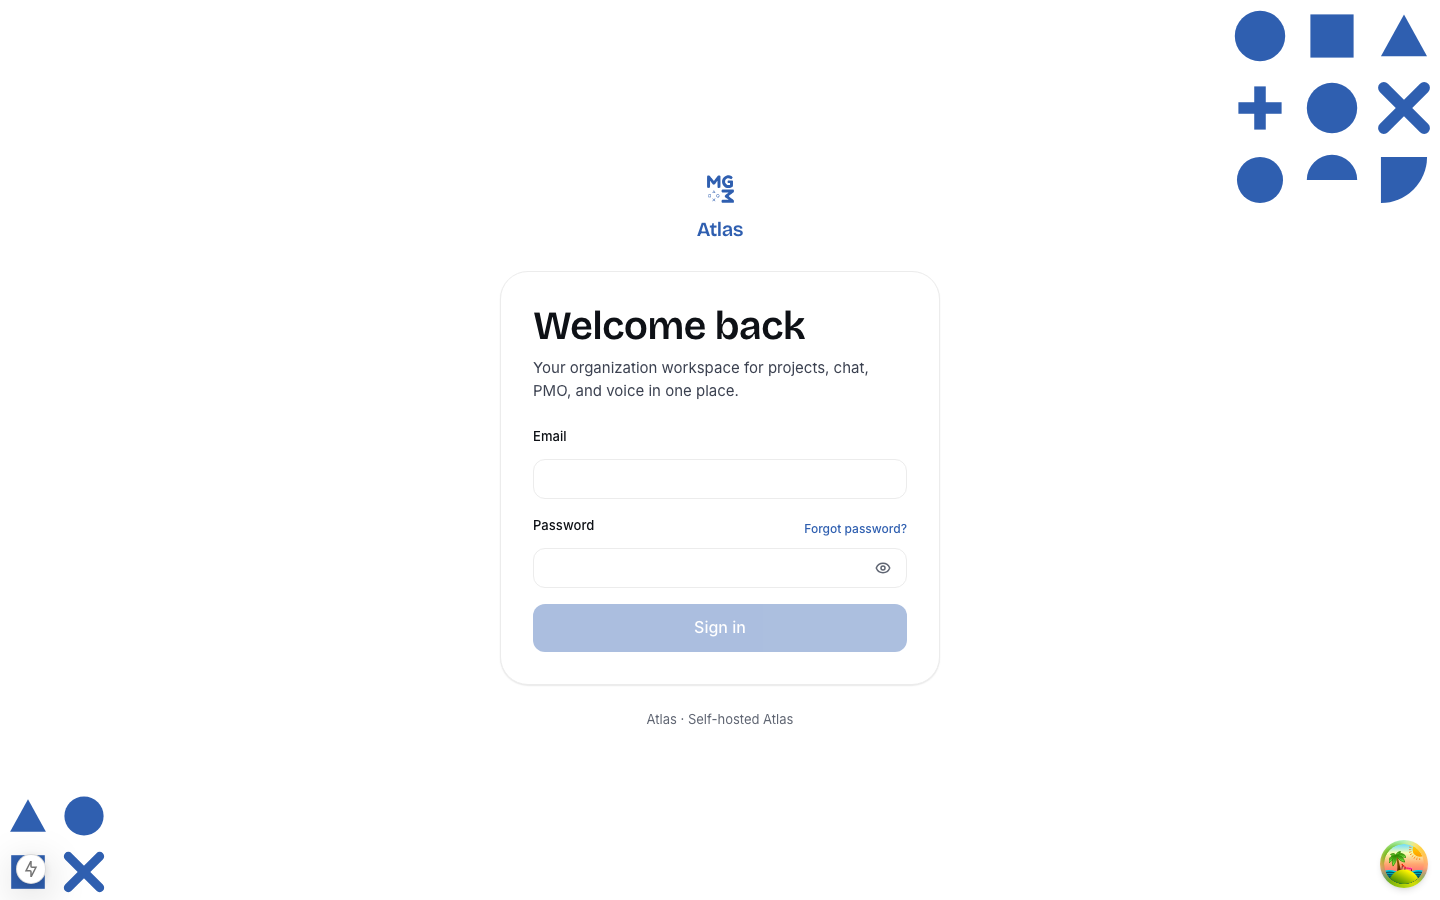
\includegraphics[width=0.485\linewidth]{assets/screenshots/curated/auth-login.png}}\hfill
\subfloat[Halaman ringkasan proyek, dengan sampul yang dibuat otomatis dari data proyek itu sendiri.]{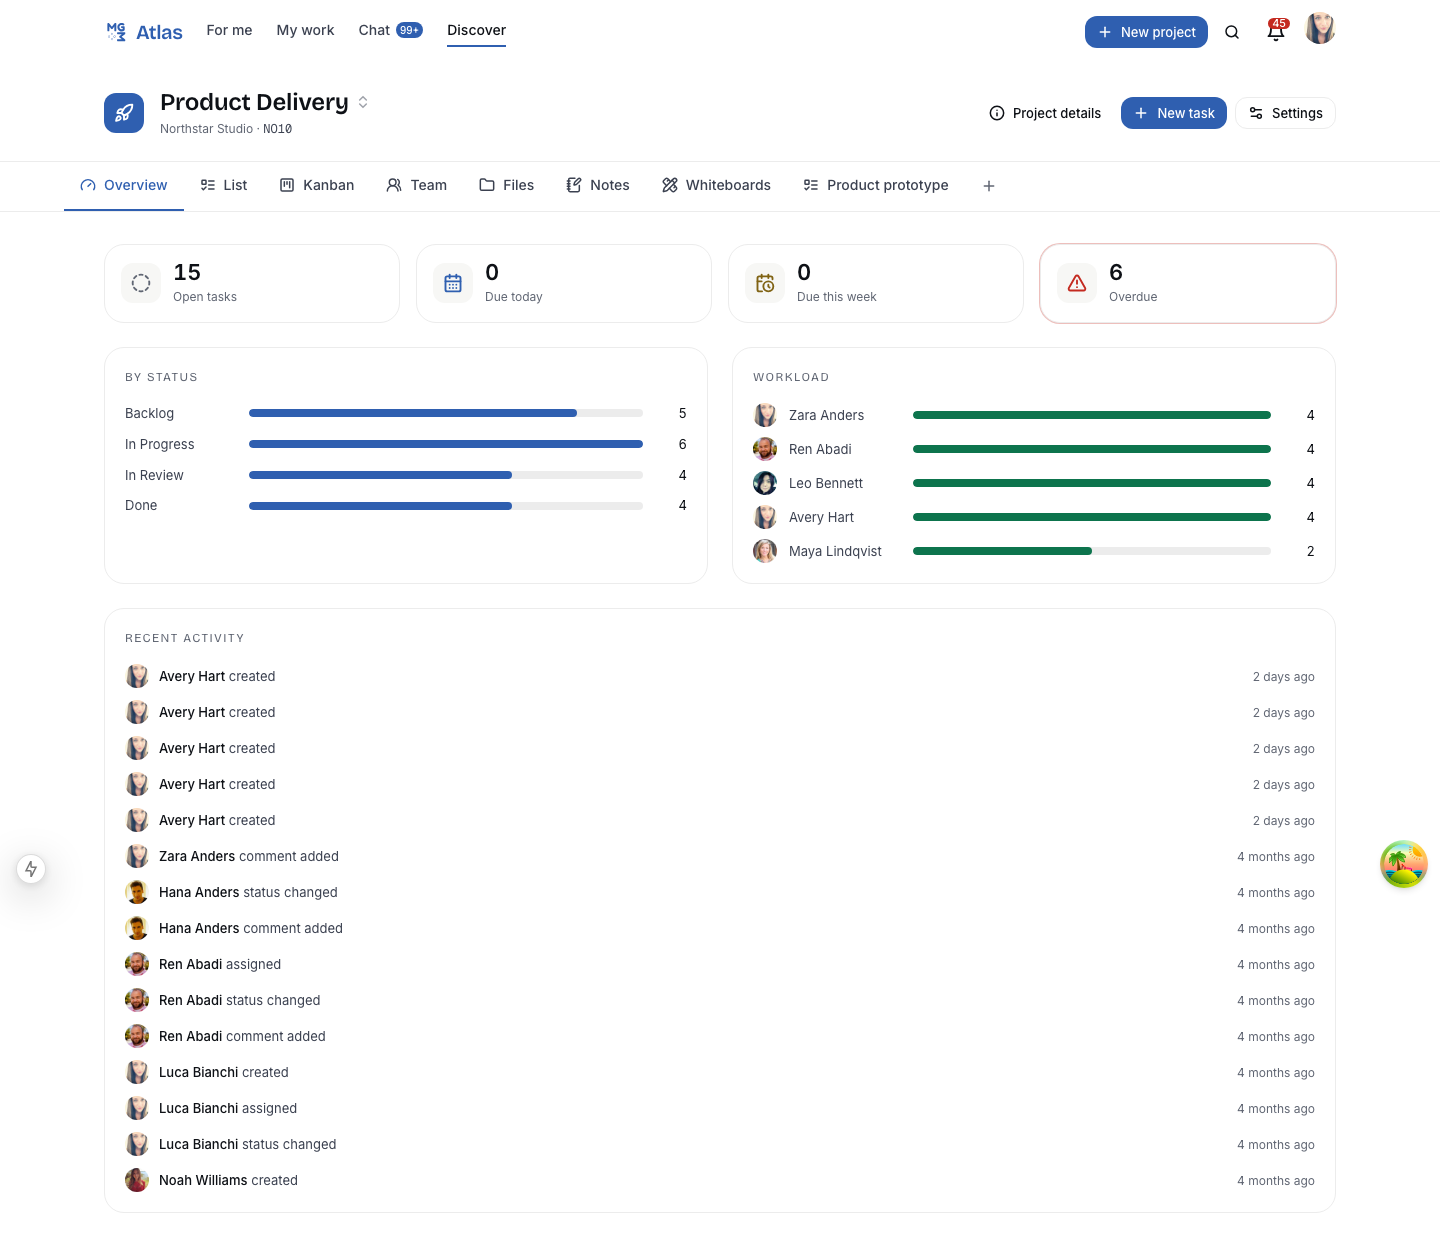
\includegraphics[width=0.485\linewidth]{assets/screenshots/curated/project-overview.png}}
\caption{Halaman masuk dan ringkasan proyek.}
\label{fig:mockup-login-project}
\end{figure*}

\FloatBarrier
\begin{figure*}[t]
\centering
\subfloat[Konsol admin: pengelolaan pengguna di luar panel Godmode.]{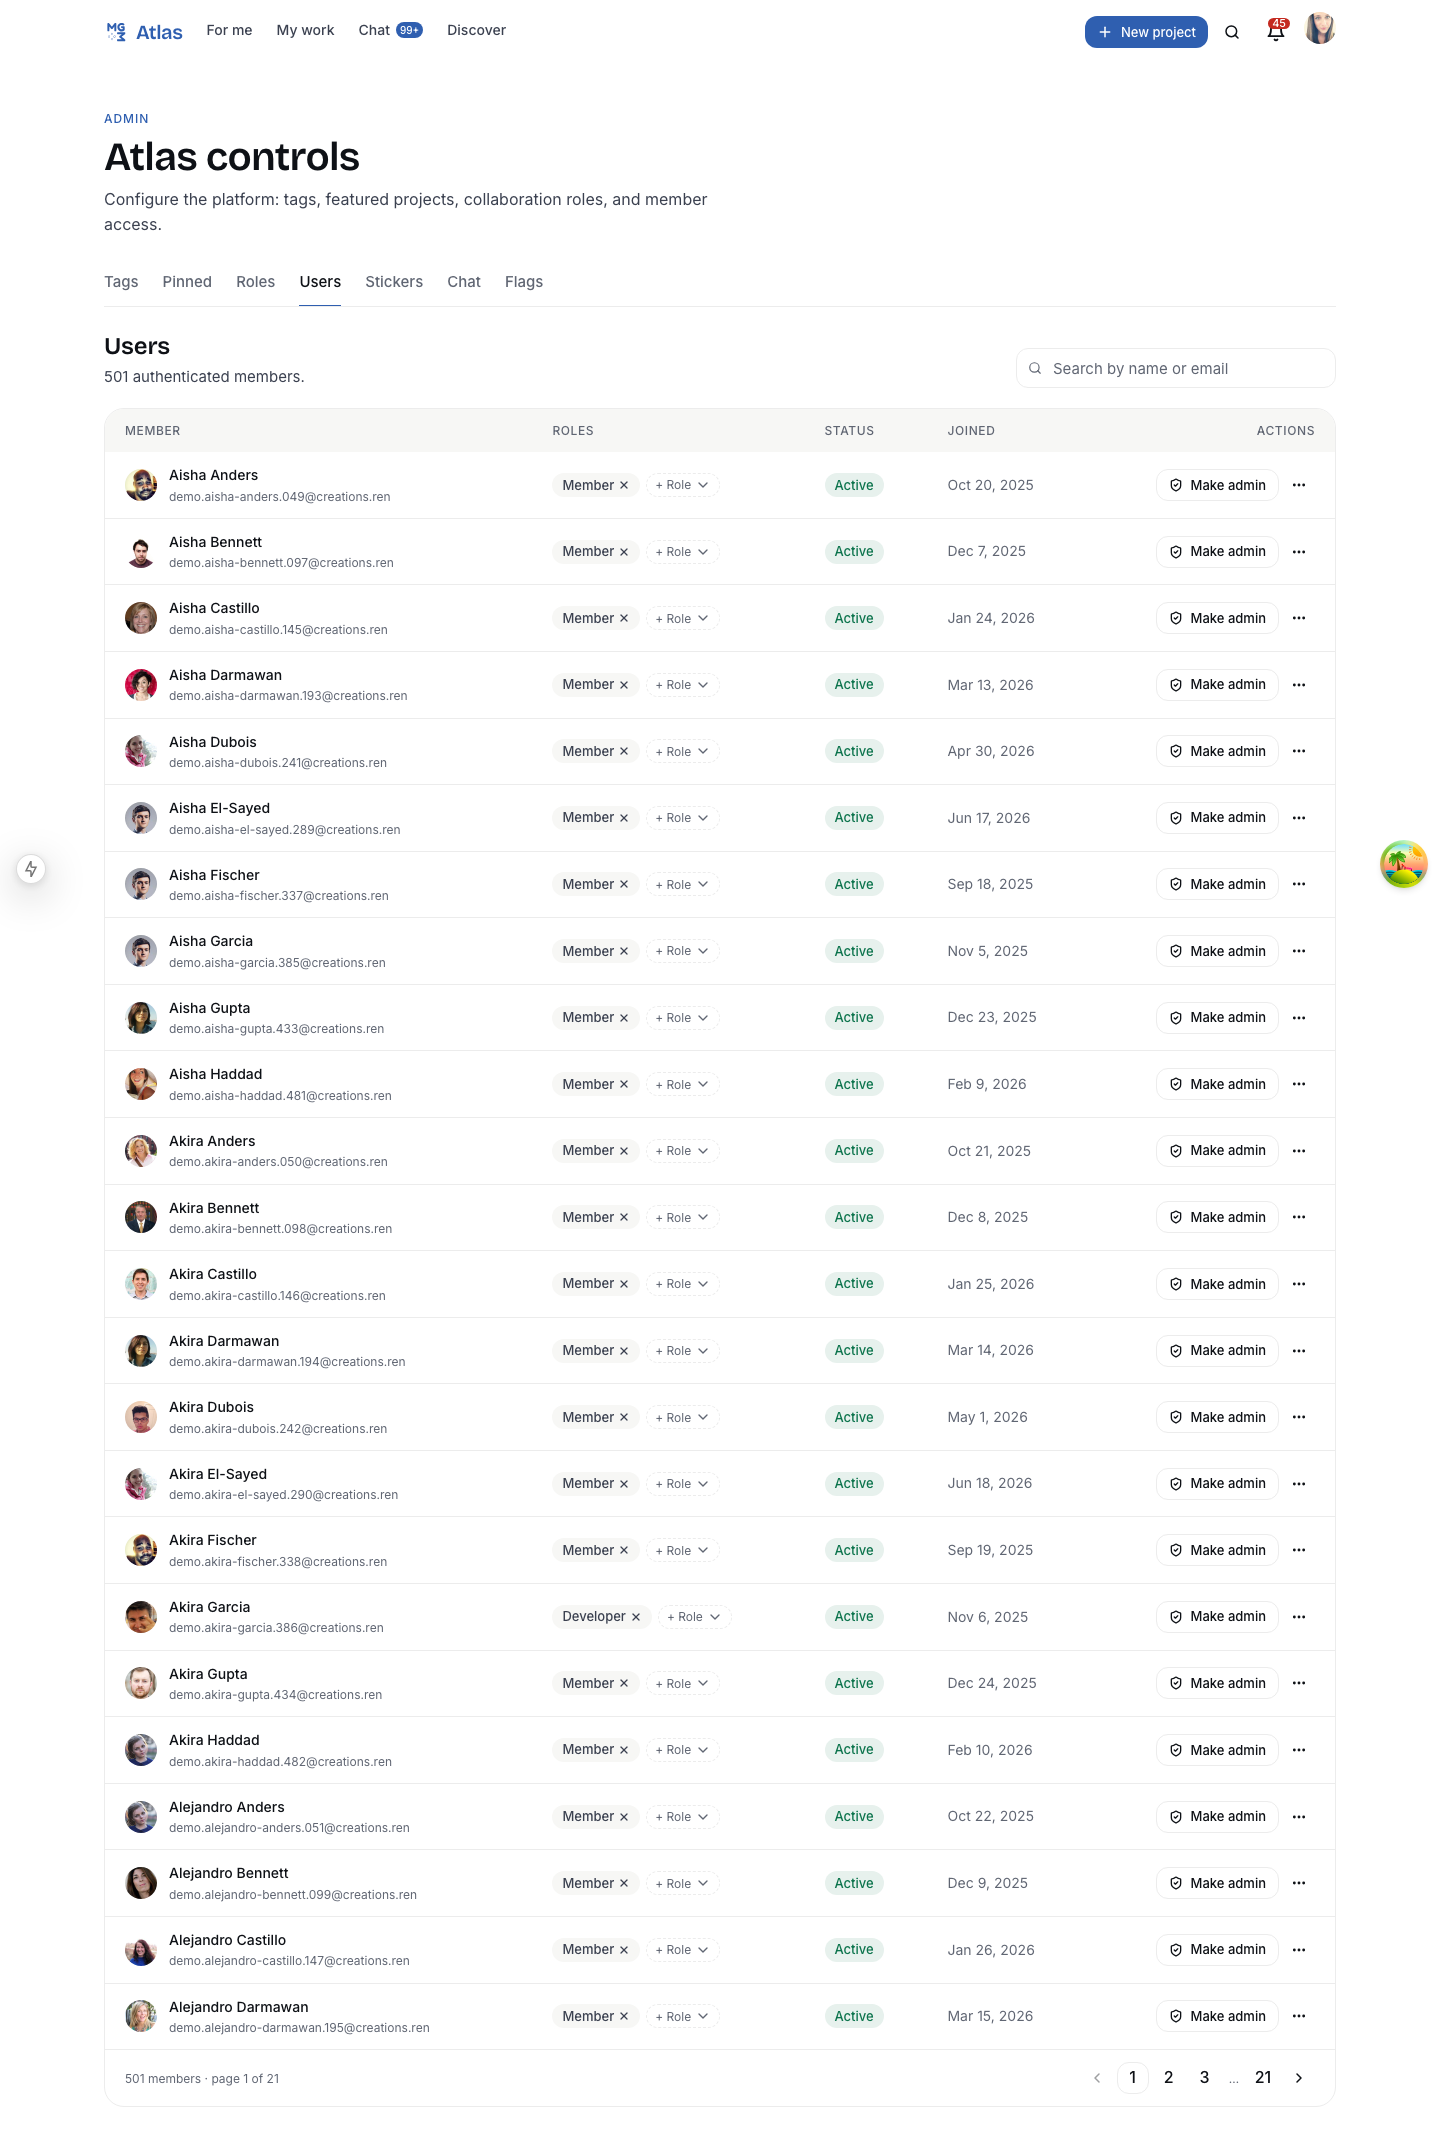
\includegraphics[width=0.485\linewidth]{assets/screenshots/curated/admin-users.png}}\hfill
\subfloat[Konfigurasi SSO institusi (OIDC/SAML) tanpa biaya tambahan.]{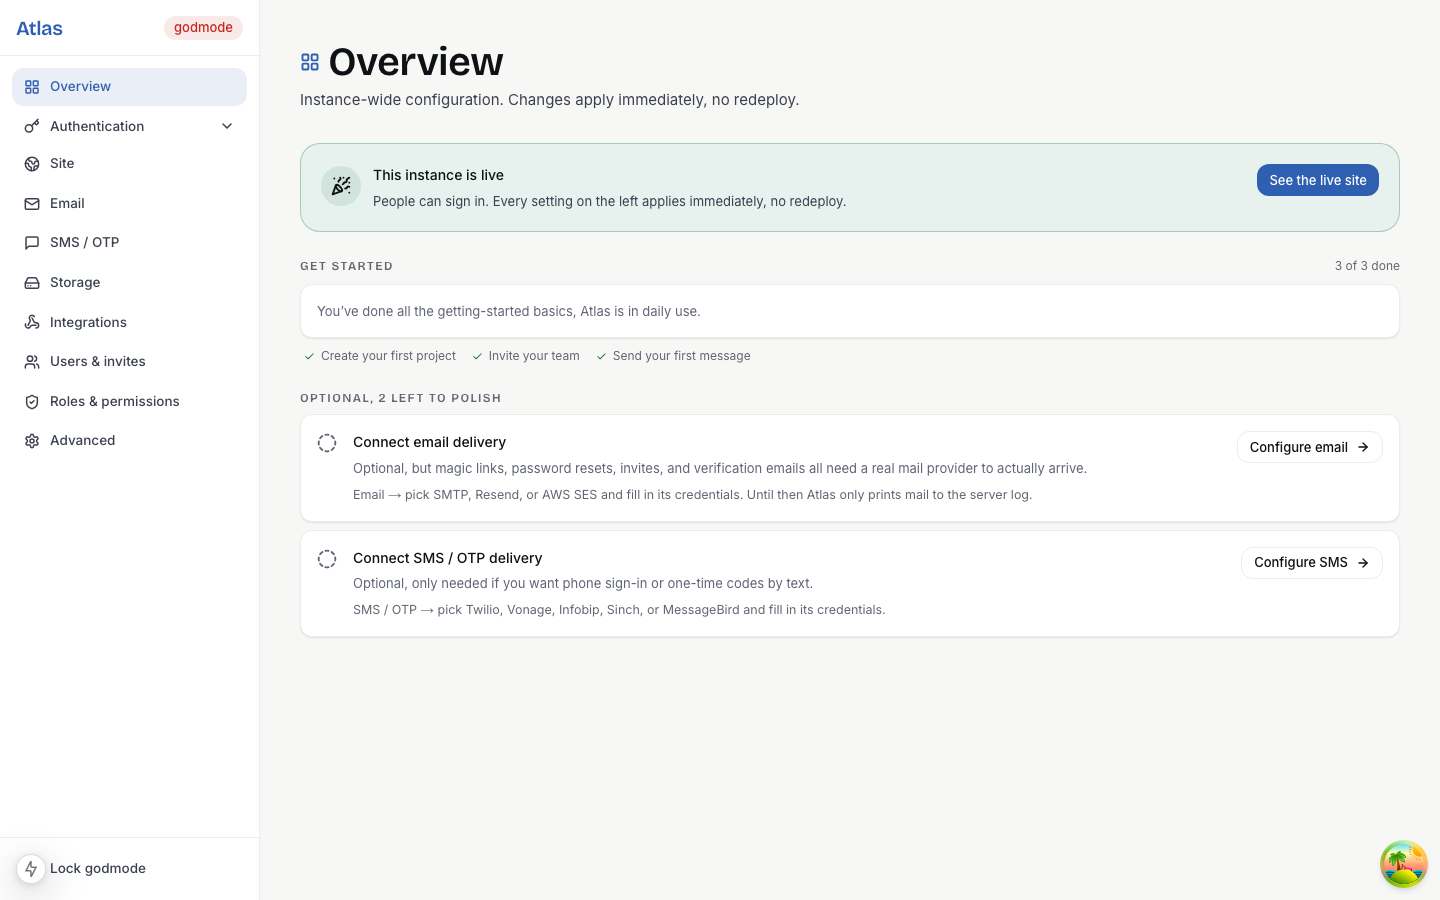
\includegraphics[width=0.485\linewidth]{assets/screenshots/curated/godmode-sso.png}}
\caption{Konsol admin dan konfigurasi SSO.}
\label{fig:mockup-admin-sso}
\end{figure*}

\FloatBarrier
\subsection{Responsif di layar ponsel}

Seluruh antarmuka melewati audit responsif lintas breakpoint (360 hingga 1920px), termasuk navigasi yang berubah jadi \textit{drawer} pada layar sempit dan target sentuh minimal 36px.

\begin{figure*}[t]
\centering
\subfloat[Discover]{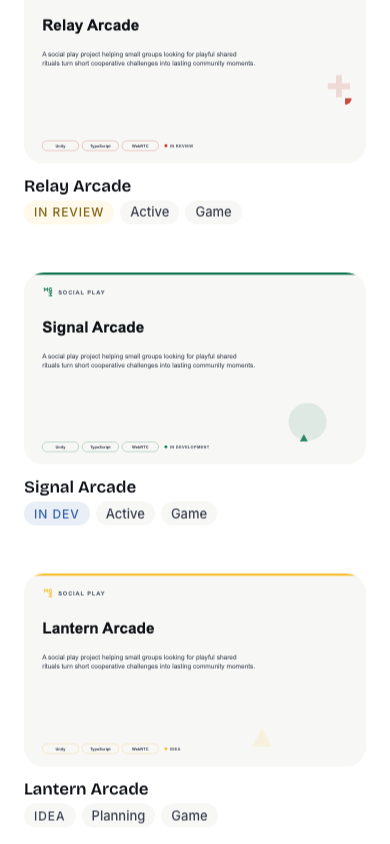
\includegraphics[width=0.31\linewidth]{assets/screenshots/curated/mobile-dashboard.png}}\hfill
\subfloat[Kanban]{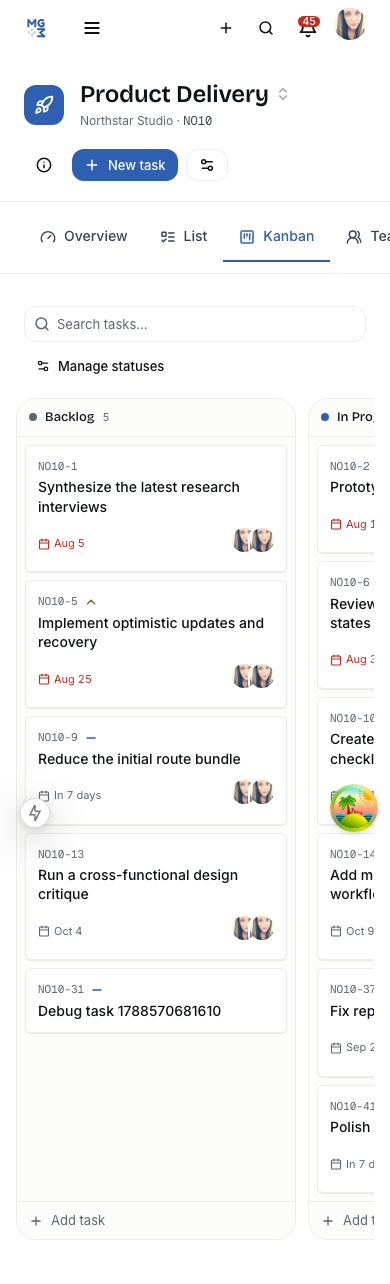
\includegraphics[width=0.31\linewidth]{assets/screenshots/curated/mobile-kanban.png}}\hfill
\subfloat[Chat]{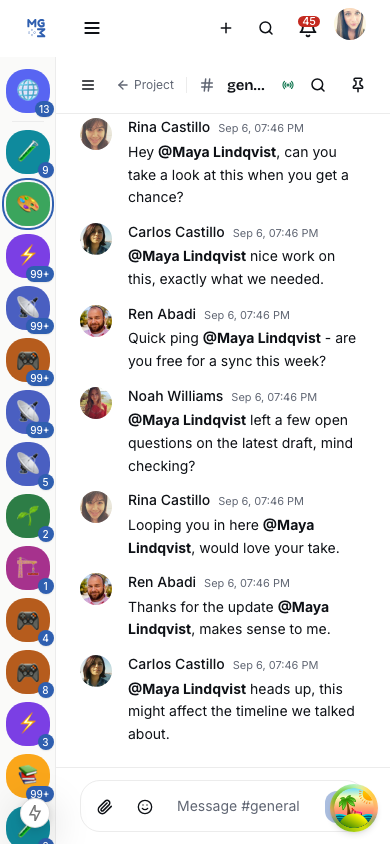
\includegraphics[width=0.31\linewidth]{assets/screenshots/curated/mobile-chat.png}}
\caption{Tiga tampilan Atlas di viewport ponsel (390px).}
\label{fig:mobile}
\end{figure*}

\FloatBarrier
